\documentclass{article}
\usepackage[english]{babel}
\usepackage[utf8]{inputenc}
\usepackage{fancyhdr}
\usepackage{geometry}
\usepackage{amsmath}
\usepackage{enumitem}
\usepackage{tcolorbox}
\usepackage{graphicx}

\geometry{letterpaper, portrait, margin=1in}
\graphicspath{ {images/}  }
\pagestyle{fancy}
\fancyhf{}
\lhead{Keerthik Muruganandam}
\rhead{Written Work 9}


\begin{document}

\textbf{(9.1)} Find $\deriv{y}\sin^{-1}{xy} = y^2-x$. Once you have found $\dfrac{dy}{dx}$, do not simplify your answer.
\[\frac{dy}{dx}\sin^{-1}{xy}=y^2-x\]
\[\frac{y+xy\prime}{\sqrt{1-x^2y^2} }= 2yy\prime-1\]
\[y+xy\prime =\sqrt{1-x^2y^2} (2yy\prime-1)\]
\[y+ \sqrt{1-x^2y^2} = (2yy\prime)\sqrt{1-x^2y^2}-xy\prime=\]
\[(2y\sqrt{1-x^2y^2}-x)y\prime\]
\[y\prime(x) = \frac{y+ \sqrt{1-x^2y^2}}{2y\sqrt{1-x^2y^2}-x}\]

\textbf{(9.2)} Find $\dfrac{dy}{dx}$ if $x^y=y^x$.
\[\frac{dy}{dx}x^y=y^x\]
\[\frac{dy}{dx}y\ln{x}=x\ln{y}\]
\[y\prime\ln{x}+\frac{y}{x}=\ln{y}+\frac{xy\prime}{y}\]
\[\frac{y}{x}-\ln{y}=\frac{xy\prime}{y}-y\prime\ln{x}=\]
\[(\frac{x}{y}-\ln{x})y\prime\]
\[y\prime(x)=\frac{\frac{y}{x}-\ln{y}}{\frac{x}{y}-\ln{x}}\]

\textbf{(9.3)} Let $f(x) = \tan^{-1}{x^2}$. \\

\indent
\indent
(a) Find $f^{\prime}(x)$ and $f^{\prime\prime}(x)$.
\[\frac{dy}{dx}y=\tan^{-1}{x^2}\]
\begin{tcolorbox}[colback=white]
\[y\prime(x)=\frac{2x}{x^4+1}\]
\end{tcolorbox}
\[y\prime\prime(x)=\frac{2\cdot(x^4+1)-(4x^3)(2x)}{{(x^4+1)}^2}\]
\begin{tcolorbox}[colback=white]
\[y\prime\prime(x)=\frac{2-6x^4}{{(x^4+1)}^2}\]
\end{tcolorbox} 
\begin{center}
cont. on next page $\rightarrow$
\end{center}


\newpage
\indent
\indent
(b) Use your answers from part (a) to determine if $f(x)$ is increasing, decreasing, concave
up, and/or concave down at the point $(-1,\dfrac{\pi}{4})$.
\[y\prime(-1)=\frac{2\cdot(-1)}{{(-1)}^4+1}=\]
\[-1\]
\begin{tcolorbox}[colback=white]
\center
$f(x)$ is decreasing at $(-1,\frac{\pi}{4})$.
\end{tcolorbox}
\[y\prime\prime(-1)=\frac{2-6{(-1)}^4}{{({(-1)}^4+1)}^2}=\]
\[\frac{-4}{4}=-1\]
\begin{tcolorbox}[colback=white]
\center
$f(x)$ is concave down at $(-1,\frac{\pi}{4})$.
\end{tcolorbox}
\newpage

\textbf{(9.4) Professional Problem} \\
\indent \indent (a) Use implicit differentiation to show that
\[{(f^{-1})}^{\prime}(x)=\frac{1}{f^{\prime}(f^{-1}(x))}\]
\indent \indent provided that the denominator isn't zero. \\
\indent \indent (b) Sketch $f(x)= \sqrt{x+e^x}$, then explain why it's plausible to believe $f^{-1}(x)$ exists.\\
\indent \indent (c) What do you need to show to prove $f^{-1}(x)$ exists.\\
\indent \indent (d) Find $f^{-1}(1)$.\\
\indent \indent (e) Use your formula from (a) to evaluate ${(f^{-1})}^\prime(1)$. \\
\newline
\newline

We know that
\[f(f^{-1}(x))=x\text{.}\]
If we differentiate both sides using the Chain Rule, we get
\[f^{\prime}(f^{-1}(x))\cdot(f^{-1})^{\prime}(x)=1\text{.}\]
After isolating $(f^{-1})^{\prime}(x)$, the equation becomes
\[(f^{-1})^{\prime}(x)=\frac{1}{f^{\prime}(f^{-1}(x)}\text{.}\]
The graph of $\sqrt{x+e^x}$ is \\
\begin{figure}[h]
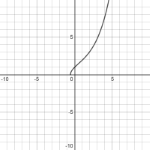
\includegraphics[scale=1.33333333333333333333333333333333333333333333333333333333333333333333333333333333333333333333333333]{graph1}.
\centering
\end{figure} \\
It is plausible to believe that $f^{-1}(x)$ exists from the graph because the function looks like a one-to-one function because the function seems to be ever-increasing. To prove that $f^{-1}(x)$ exists, the function $f$ must be one-to-one. i=In other words, $f^{\prime}$ must never change sign or the function will start increasing/decreasing meaning the function won't be one-to-one anymore. To solve for $f^{-1}(1)$, we simply take the fact that 
\[f(0)=1\text{,}\]
therefore
\[f^{-1}(1)=0\text{.}\]
Using the equation from (a), we get
\[\frac{1}{f^{\prime}(0)}=\]
\[\frac{1}{\frac{1 + e^0}{2 \sqrt{e^0 + 0}}}=\frac{1}{\frac{2}{2}}=1\text{.}\]
Thus the function $(f^{-1})^{\prime}(x)=1$

%pls I need to finish
 
\end{document} 
